\section{uart.h File Reference}
\label{uart_8h}\index{uart.h@{uart.h}}


This graph shows which files directly or indirectly include this file:\begin{figure}[H]
\begin{center}
\leavevmode
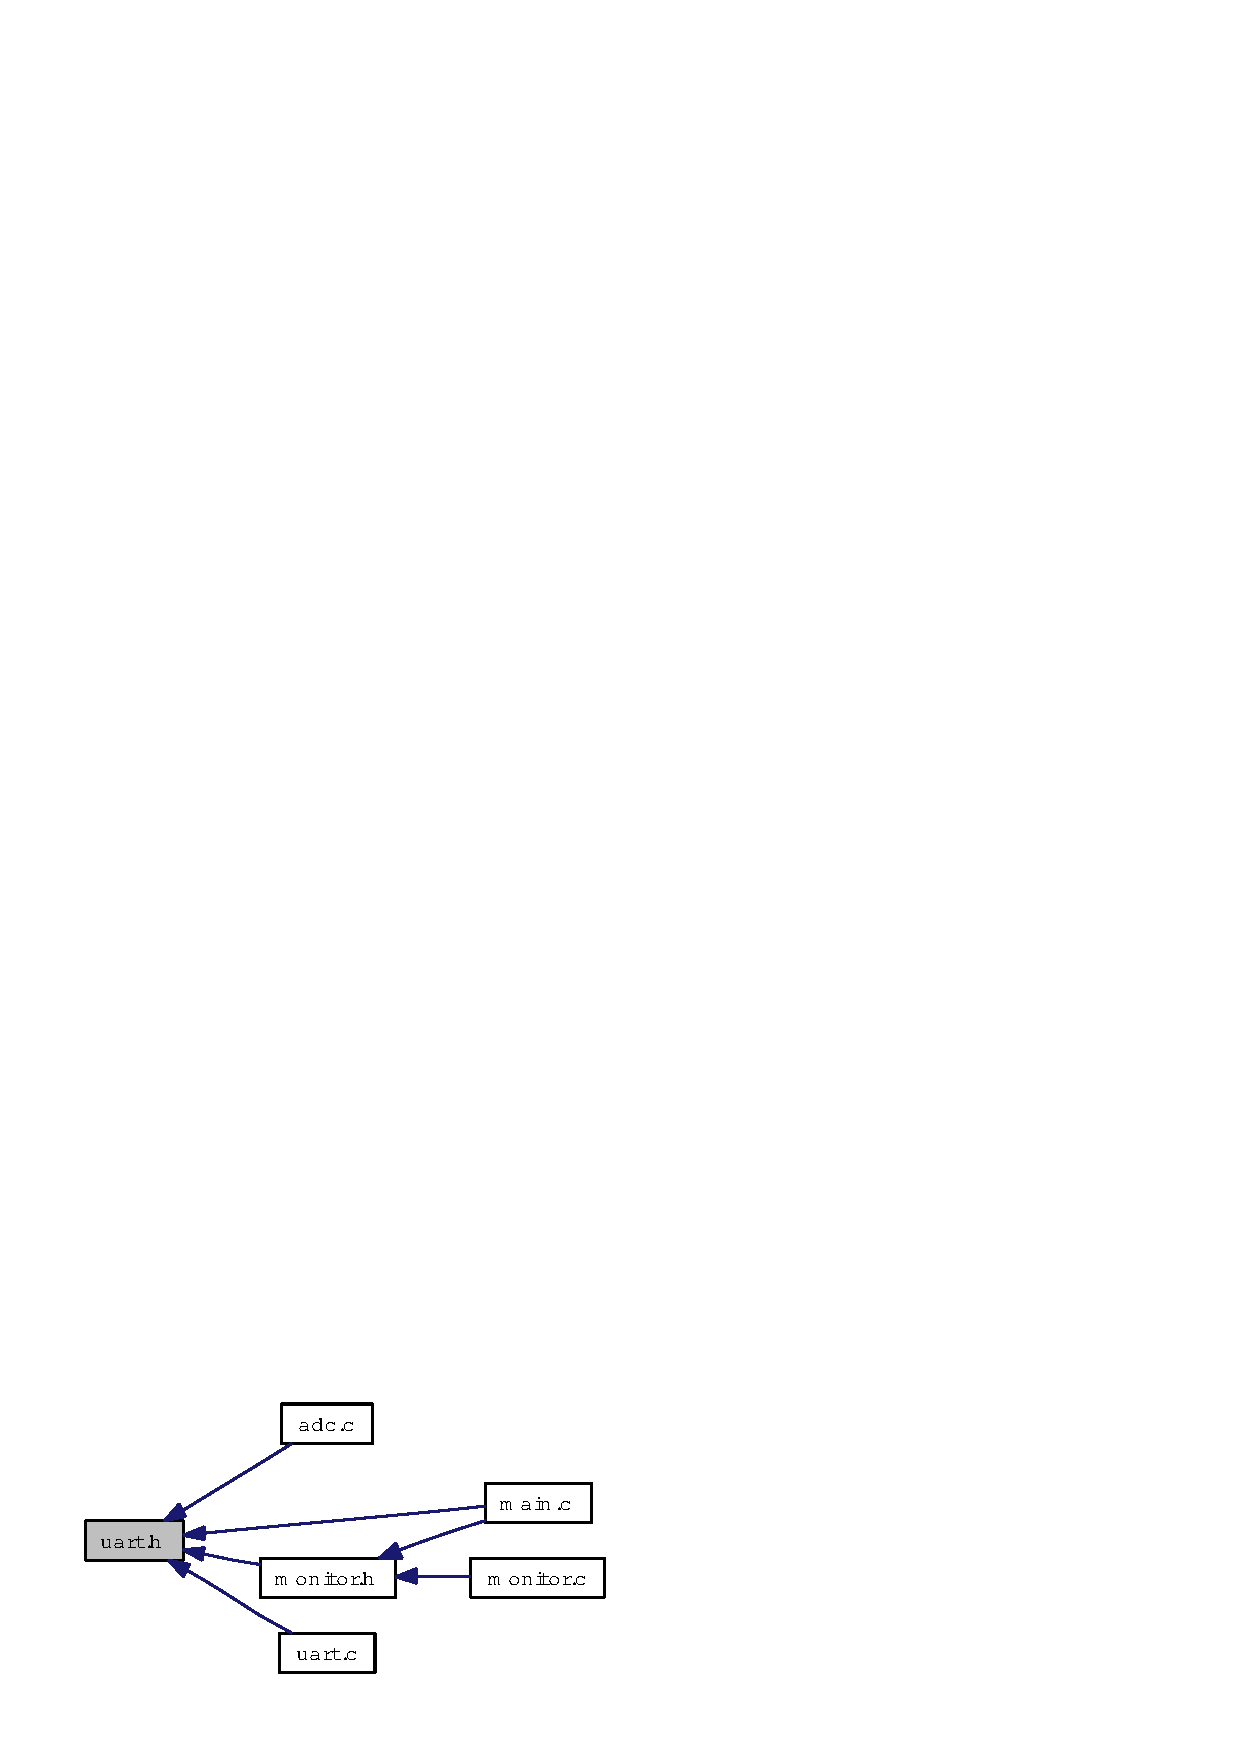
\includegraphics[width=147pt]{uart_8h__dep__incl}
\end{center}
\end{figure}
\subsection*{Defines}
\begin{CompactItemize}
\item 
\#define {\bf UART\_\-BAUD\_\-SELECT}(baud\-Rate, xtal\-Cpu)~((xtal\-Cpu)/((baud\-Rate)$\ast$16l)-1)
\begin{CompactList}\small\item\em UART Baudrate Expression. \item\end{CompactList}\item 
\#define {\bf UART\_\-BAUD\_\-SELECT\_\-DOUBLE\_\-SPEED}(baud\-Rate, xtal\-Cpu)~(((xtal\-Cpu)/((baud\-Rate)$\ast$8l)-1)$|$0x8000)
\begin{CompactList}\small\item\em UART Baudrate Expression for ATmega double speed mode. \item\end{CompactList}\item 
\#define {\bf UART\_\-RX\_\-BUFFER\_\-SIZE}~32
\item 
\#define {\bf UART\_\-TX\_\-BUFFER\_\-SIZE}~32
\item 
\#define {\bf UART\_\-FRAME\_\-ERROR}~0x0800
\item 
\#define {\bf UART\_\-OVERRUN\_\-ERROR}~0x0400
\item 
\#define {\bf UART\_\-BUFFER\_\-OVERFLOW}~0x0200
\item 
\#define {\bf UART\_\-NO\_\-DATA}~0x0100
\item 
\#define {\bf uart\_\-puts\_\-P}(\_\-\_\-s)~uart\_\-puts\_\-p(PSTR(\_\-\_\-s))
\begin{CompactList}\small\item\em Macro to automatically put a string constant into program memory. \item\end{CompactList}\item 
\#define {\bf uart1\_\-puts\_\-P}(\_\-\_\-s)~uart1\_\-puts\_\-p(PSTR(\_\-\_\-s))
\begin{CompactList}\small\item\em Macro to automatically put a string constant into program memory. \item\end{CompactList}\end{CompactItemize}
\subsection*{Functions}
\begin{CompactItemize}
\item 
void {\bf init\_\-uart} (void)
\item 
void {\bf uart\_\-init} (unsigned int baudrate)
\begin{CompactList}\small\item\em Initialize UART and set baudrate. \item\end{CompactList}\item 
unsigned int {\bf uart\_\-getc} (void)
\begin{CompactList}\small\item\em Get received byte from ringbuffer. \item\end{CompactList}\item 
void {\bf uart\_\-putc} (unsigned char data)
\begin{CompactList}\small\item\em Put byte to ringbuffer for transmitting via UART. \item\end{CompactList}\item 
void {\bf uart\_\-puts} (const char $\ast$s)
\begin{CompactList}\small\item\em Put string to ringbuffer for transmitting via UART. \item\end{CompactList}\item 
void {\bf uart\_\-puts\_\-p} (const char $\ast$s)
\begin{CompactList}\small\item\em Put string from program memory to ringbuffer for transmitting via UART. \item\end{CompactList}\item 
void {\bf uart1\_\-init} (unsigned int baudrate)
\begin{CompactList}\small\item\em Initialize USART1 (only available on selected ATmegas). \item\end{CompactList}\item 
unsigned int {\bf uart1\_\-getc} (void)
\begin{CompactList}\small\item\em Get received byte of USART1 from ringbuffer. (only available on selected ATmega). \item\end{CompactList}\item 
void {\bf uart1\_\-putc} (unsigned char data)
\begin{CompactList}\small\item\em Put byte to ringbuffer for transmitting via USART1 (only available on selected ATmega). \item\end{CompactList}\item 
void {\bf uart1\_\-puts} (const char $\ast$s)
\begin{CompactList}\small\item\em Put string to ringbuffer for transmitting via USART1 (only available on selected ATmega). \item\end{CompactList}\item 
void {\bf uart1\_\-puts\_\-p} (const char $\ast$s)
\begin{CompactList}\small\item\em Put string from program memory to ringbuffer for transmitting via USART1 (only available on selected ATmega). \item\end{CompactList}\end{CompactItemize}
